% Slides for the talk at HessPL on September 11, 2014.
% http://ps-mr.github.io/hesspl-2014/

\documentclass{beamer}
\usetheme{default}
\setbeamertemplate{navigation symbols}{}
\setbeamertemplate{footline}[frame number]

\usepackage[utf8x]{inputenc}
\usepackage{tikz}
\usetikzlibrary{shapes,arrows,positioning}
\usepackage{listings}
\lstset{
  basicstyle=\ttfamily,
  columns=fullflexible,
  keepspaces=true,
}
\usepackage{syntax}

\title{A Language for the Specification and Efficient Implementation
  of Type Systems}
\author{Pascal Wittmann}
\institute{TU Darmstadt}
\date{September 11, 2014}

\begin{document}

\begin{frame}[plain]
  \titlepage{}
\end{frame}

\begin{frame}
  \frametitle{Motivation}
  \begin{itemize}
  \item Type systems provide
    \begin{itemize}
    \item static approximation of programs semantics
    \item means to establish and enforce abstraction barriers
    \item documentation that is always correct
    \end{itemize}
  \item Domains specific languages benefit from specialized type
    systems
  \item Gap between formal definitions of type systems and their
    implementations
  \end{itemize}
\end{frame}

\begin{frame}
  \frametitle{Research Problem}
  \begin{itemize}
  \item Design of a declarative specification language that
    \begin{itemize}
    \item is close to text-book formalisms
    \item makes it easy to use existing programming language definitions
    \end{itemize}
  \item Generate first-order formula representations of specifications
  \item Develop a type checker generator which
    \begin{itemize}
    \item is constraint-based
    \item can cope with non-syntax directed rules
    \item takes advantage of facts proven by automated theorem provers
    \end{itemize}
  \end{itemize}
  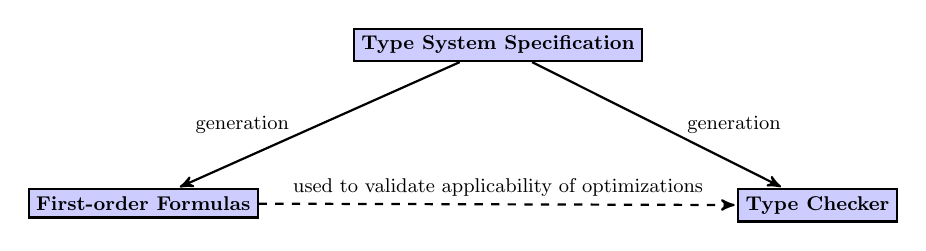
\begin{tikzpicture}[scale=.8,transform shape,->,>=stealth',shorten >=1pt,auto,align=center,node distance=5cm,thick,main node/.style={rectangle,fill=blue!20,draw,font=\small\bfseries}]
    \node[main node] (1) {Type System Specification};
    \node[main node] (2) [below left=2cm and 1.5cm of 1]  {First-order Formulas};
    \node[main node] (3) [below right=2cm and 1.5cm of 1] {Type Checker};

  \path[every node/.style={font=\small}]
  (1) edge node [outer sep=10pt,left] {generation} (2)
  (1) edge node [outer sep=10pt,right] {generation} (3);

  \path[every node/.style={font=\small}, dashed]
  (2) edge node [above] {used to validate applicability of
    optimizations} (3);
  \end{tikzpicture}
\end{frame}

\begin{frame}[allowframebreaks,fragile]
  \frametitle{Specification Language}
\begin{lstlisting}
module Typesystem

language specifications/SystemF/SystemF

contexts
TermBinding := ID{I} x Type{O}
TypeBinding := ID{I}

meta-variables 	Term "~" { Type Exp }
                Ctx "$" { TermBinding TypeBinding }
                Id "%" { ID }
                Num "&" { Int }
\end{lstlisting}
\framebreak{}
\begin{lstlisting}
judgments
TermBinding{I} "|" TypeBinding{I} "|-" Exp{I} ":" Type{O}.
Type{O} "= [" ID{I} "->" Type{I} "]" Type{I}.
ID{I} "fresh in" TypeBinding{I}.
ID{I} "!=" ID{I} is Neq.
\end{lstlisting}
\framebreak{}
\small
\begin{lstlisting}
rules

%x : ~T in $C1       @error %x "should have type" ~T
                            "but has type" {}.
=============== T-Var
$C1 | $C2 |- %x : ~T


~U = [ %x -> ~S ] ~T           @error ~U "is not" ~T "where"
                                      %x "is replaced by" ~S.
$C1 | $C2 |- ~e : all %x . ~T
============================== T-Tapp
$C1 | $C2 |- ~e [ ~S ] : ~U
\end{lstlisting}
\end{frame}

\newcommand*\selectTemplateGeneration{}
\newcommand*\selectTemplateOptimization{}
\newcommand*\selectConstraintGeneration{}
\newcommand*\selectConstraintSolving{}
\begin{frame}[label=overview]
  \frametitle{Phases of the type checker generator}
\begin{figure}
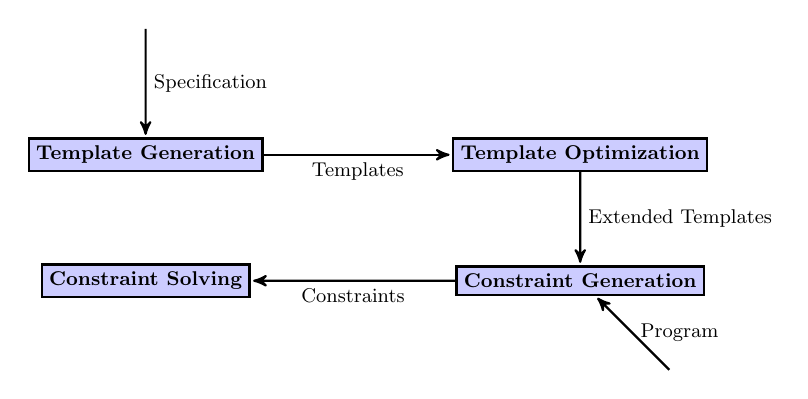
\begin{tikzpicture}[scale=.8,transform shape,->,>=stealth',shorten >=1pt,auto,align=center,node distance=2cm,
  thick,main node/.style={rectangle,fill=blue!20,draw,font=\small\bfseries}]
  \node[main node,fill=\selectTemplateGeneration] (1) {Template Generation};
  \node[main node,fill=\selectTemplateOptimization] (2) [right=3cm of 1] {Template Optimization};
  \node[main node,fill=\selectConstraintGeneration] (3) [below of=2] {Constraint Generation};
  \node[main node,fill=\selectConstraintSolving] (4) [below of=1] {Constraint Solving};
  \coordinate [below right of=3] (5);
  \coordinate [above of=1] (6);

  \path[every node/.style={font=\small}]
    (1) edge node [right, below] {Templates} (2)
    (2) edge node [right] {Extended Templates} (3)
    (5) edge node [right] {Program} (3)
    (3) edge node [right, below] {Constraints} (4)
    (6) edge node [right] {Specification} (1);
\end{tikzpicture}
\label{fig:phases}
\end{figure}
\end{frame}

\renewcommand*\selectTemplateGeneration{orange}
\againframe{overview}
\renewcommand*\selectTemplateGeneration{}

\defverbatim[colored]\lstApp{%
\begin{lstlisting}
~U = [ %x -> ~S ] ~T
$C1 | $C2 |- ~e : all %x . ~T
============================== T-Tapp
$C1 | $C2 |- ~e [ ~S ] : ~U
\end{lstlisting}
}

\defverbatim[colored]\lstAppRewritten{%
\begin{lstlisting}
$C1 | $C2 |- ~e : all %x . ~T
~U = [ %x -> ~S ] ~T
============================== T-Tapp
$C1 | $C2 |- ~e [ ~S ] : ~U
\end{lstlisting}
}

\defverbatim[colored]\lstSubst{%
\begin{lstlisting}

===================== Subst-Eq
~S = [ %x -> ~S ] %x
\end{lstlisting}
}

\defverbatim[colored]\lstSubstRewritten{%
\begin{lstlisting}
%y = %z
===================== SubstEq
~S = [ %y -> ~S ] %z
\end{lstlisting}
}

\begin{frame}[allowframebreaks, fragile]
  \frametitle{Template Generation}
  \begin{itemize}
  \item Templates are an intermediate representation of the rules
    suitable for constraint generation
  \item An excerpt of the syntax definition of a template:
  \end{itemize}

  \begin{grammar}
    <Template> ::= `Template' $\langle$Premisses$\rangle$ $\langle$Conjecture$\rangle$

    <Conjecture> ::= `Conjecture' $\langle$Judg$\rangle$ $\langle$Name$\rangle$ $\langle$Pattern$\rangle$ $\langle$Outputs$\rangle$

    <Premisses> ::= $\epsilon$ | $\langle$Premise$\rangle$ $\langle$Dependencies$\rangle$ $\langle$Premisses$\rangle$

    <Premise> ::= `Lookup' $\langle$Ctx$\rangle$ $\langle$Inputs$\rangle$ $\langle$Outputs$\rangle$ $\langle$Error$\rangle$
    \alt `Judgment' $\langle$Judg$\rangle$ $\langle$Inputs$\rangle$ $\langle$Binding$\rangle$ $\langle$Outputs$\rangle$ $\langle$Error$\rangle$
    \alt `Eq' $\langle$Term$\rangle$ $\langle$Term$\rangle$ $\langle$Error$\rangle$
    \alt `Neq' $\langle$Term$\rangle$ $\langle$Term$\rangle$ $\langle$Error$\rangle$
  \end{grammar}
\end{frame}

\begin{frame}[fragile]
  \frametitle{Template Generation II}
\begin{itemize}
\item Resolve Dependencies between premisses
  \begin{grammar}
    <Dependencies> ::= $\epsilon$ | $\langle$Judg$\rangle$ $\langle$Outputs$\rangle$ $\langle$Dependencies$\rangle$
  \end{grammar}
\item Resolve implicit equalities
\end{itemize}

\begin{figure}
\begin{lstlisting}
TermBinding{I} "|" TypeBinding{I} "|-" Exp{I} ":" Type{O}.
Type{O} "= [" ID{I} "->" Type{I} "]" Type{I}.
\end{lstlisting}

\only<1>{\lstApp}
\only<2->{\lstAppRewritten}
\only<1,2>{\lstSubst}
\only<3->{\lstSubstRewritten}
%% TODO: Verbatim does not work in captions
\caption{Premisses depend on each other in T-Tapp and
  Subst-Eq has an implicit equality}
\end{figure}
\end{frame}

\renewcommand*\selectTemplateOptimization{orange}
\againframe{overview}
\renewcommand*\selectTemplateOptimization{}

\begin{frame}[allowframebreaks, fragile]
  \frametitle{Template Optimization}
  \begin{itemize}
  \item In contrast to the rules templates are normalized
  \item Templates can still contain redundancies and
    non-syntax-directed rules
  \item We use a first-order formula representation of the templates
    to prove properties that allow to remove redundancies and to make
    templates syntax directed
  \item The first-order formula representation of a template looks
    roughly like this
    \begin{align}
      \forall FV(p_1,\dots, p_n, c) .& p_1 \land \dots \land p_n
      \implies c
    \end{align}
    where $p_i$ and $c$ are propositions representing the premisses
    respectively the conclusion
  \end{itemize}

\framebreak{}

  \begin{itemize}
  \item A template is \textit{when-ambiguous} if there is an other
    template such that there is at least one term that matches the
    conclusion of both templates
  \item If the set of terms is equal, they are \textit{which-ambiguous}
\begin{figure}
\begin{lstlisting}
~T <: ~S
{ $R } <: { $U }
=============================== S-depth
{ %l : ~T $R } <: { %l : ~S $U }

{ $R } <: { $S }
=============================== S-width
{ %l : ~T $R } <: { %l : ~T $S}
\end{lstlisting}
\caption{Which-ambiguity between depth and width subtyping rules of records}
\end{figure}
\end{itemize}

\framebreak{}

\begin{itemize}
\item We also try to solve a certain class of when-ambiguities, namely
  relations that do not involve contexts
\item Look at the subtyping relation \verb|Type{I} "<:" Type{I}|,
  where \verb|Type| contains arrow types and the base type \verb|int|
  \begin{minipage}[b]{.4\linewidth}
\begin{lstlisting}
======== S-refl
~T <: ~T
\end{lstlisting}
  \end{minipage}
  \begin{minipage}[b]{.4\linewidth}
\begin{lstlisting}
~S <: ~Y
~Y <: ~T
======== S-trans
~S <: ~T
\end{lstlisting}
  \end{minipage}
  \begin{lstlisting}
~T1 <: ~S1
~S2 <: ~T2
======================== S-arrow
~S1 -> ~S2 <: ~T1 -> ~T2
  \end{lstlisting}
\end{itemize}

\framebreak{}

\begin{itemize}
\item Ambiguities are captured in the template language by \verb|Fork|
\item \verb|Fork| groups templates, such that they match at least on
  one common term
\item After the last optimization step forks are sorted by $<$
  \begin{align}
    t_1 < t_2 \iff m(t_1) \supseteq m(t_2)
  \end{align}
  where $m(t)$ computes the set of terms that match the conclusion of $t$
\end{itemize}
\end{frame}

\renewcommand*\selectConstraintGeneration{orange}
\againframe{overview}
\renewcommand*\selectConstraintGeneration{}

\begin{frame}
  \frametitle{Constraint Generation}
  \begin{itemize}
  \item The constraint language
  \begin{grammar}
    <Constraint> ::= `CFail' $\langle$Error$\rangle$
    \alt `CEq' $\langle$Term$\rangle$ $\langle$Term$\rangle$ $\langle$Error$\rangle$
    \alt `CNeq' $\langle$Term$\rangle$ $\langle$Term$\rangle$ $\langle$Error$\rangle$
  \end{grammar}
  \item Contexts are stored has hash tables
  \item As a fist step constraints are initialized
  \item Then a template that matches the input and the current state
    of the contexts is fetched
  \item If the selected template is a fork, the contained templates
    are processed from left to right until the first resulting
    constraint set unifies
  \item Otherwise the context is modified accordingly to the
    conclusion, the patterns of the premisses are instantiated, the
    premisses are evaluated and then the emitted constraints are
    collected
  \end{itemize}
\end{frame}

\renewcommand*\selectConstraintSolving{orange}
\againframe{overview}
\renewcommand*\selectConstraintSolving{}

\begin{frame}
  \frametitle{Constraint Solving}
  \begin{itemize}
  \item Constraints are solved by Robinson unification
  \item If a constraint cannot be unified the error message is recorded
  \item During unification a most general unifier (mgu) is computed
  \item On a successful unification the mgu is applied to the output
    of the constraint generation
  \item Otherwise the mgu is applied to the collected error messages
  \end{itemize}
\end{frame}

\begin{frame}
  \frametitle{Conclusion}
  \begin{itemize}
  \item We presented
    \begin{itemize}
    \item a high-level specification language for type systems in SDF
    \item a template language that normalizes typing rules
    \item methods to optimize templates
    \item a generic constraint-based type checker that uses templates
      as input
    \item a first-order formula representation for type systems
    \end{itemize}
  \item We applied the results to
    \begin{itemize}
    \item programming languages like SystemF and variants of the lambda
      calculus with subtyping
    \item security type systems from information flow
      security~\cite{Volpano:1996:STS:353629.353648}
    \end{itemize}
  \end{itemize}
\end{frame}

\begin{frame}
  \frametitle{References}
  \bibliographystyle{amsalpha}
  \bibliography{../report/bibliography.bib}
\end{frame}

\end{document}